\begin{figure}[H]
\centering
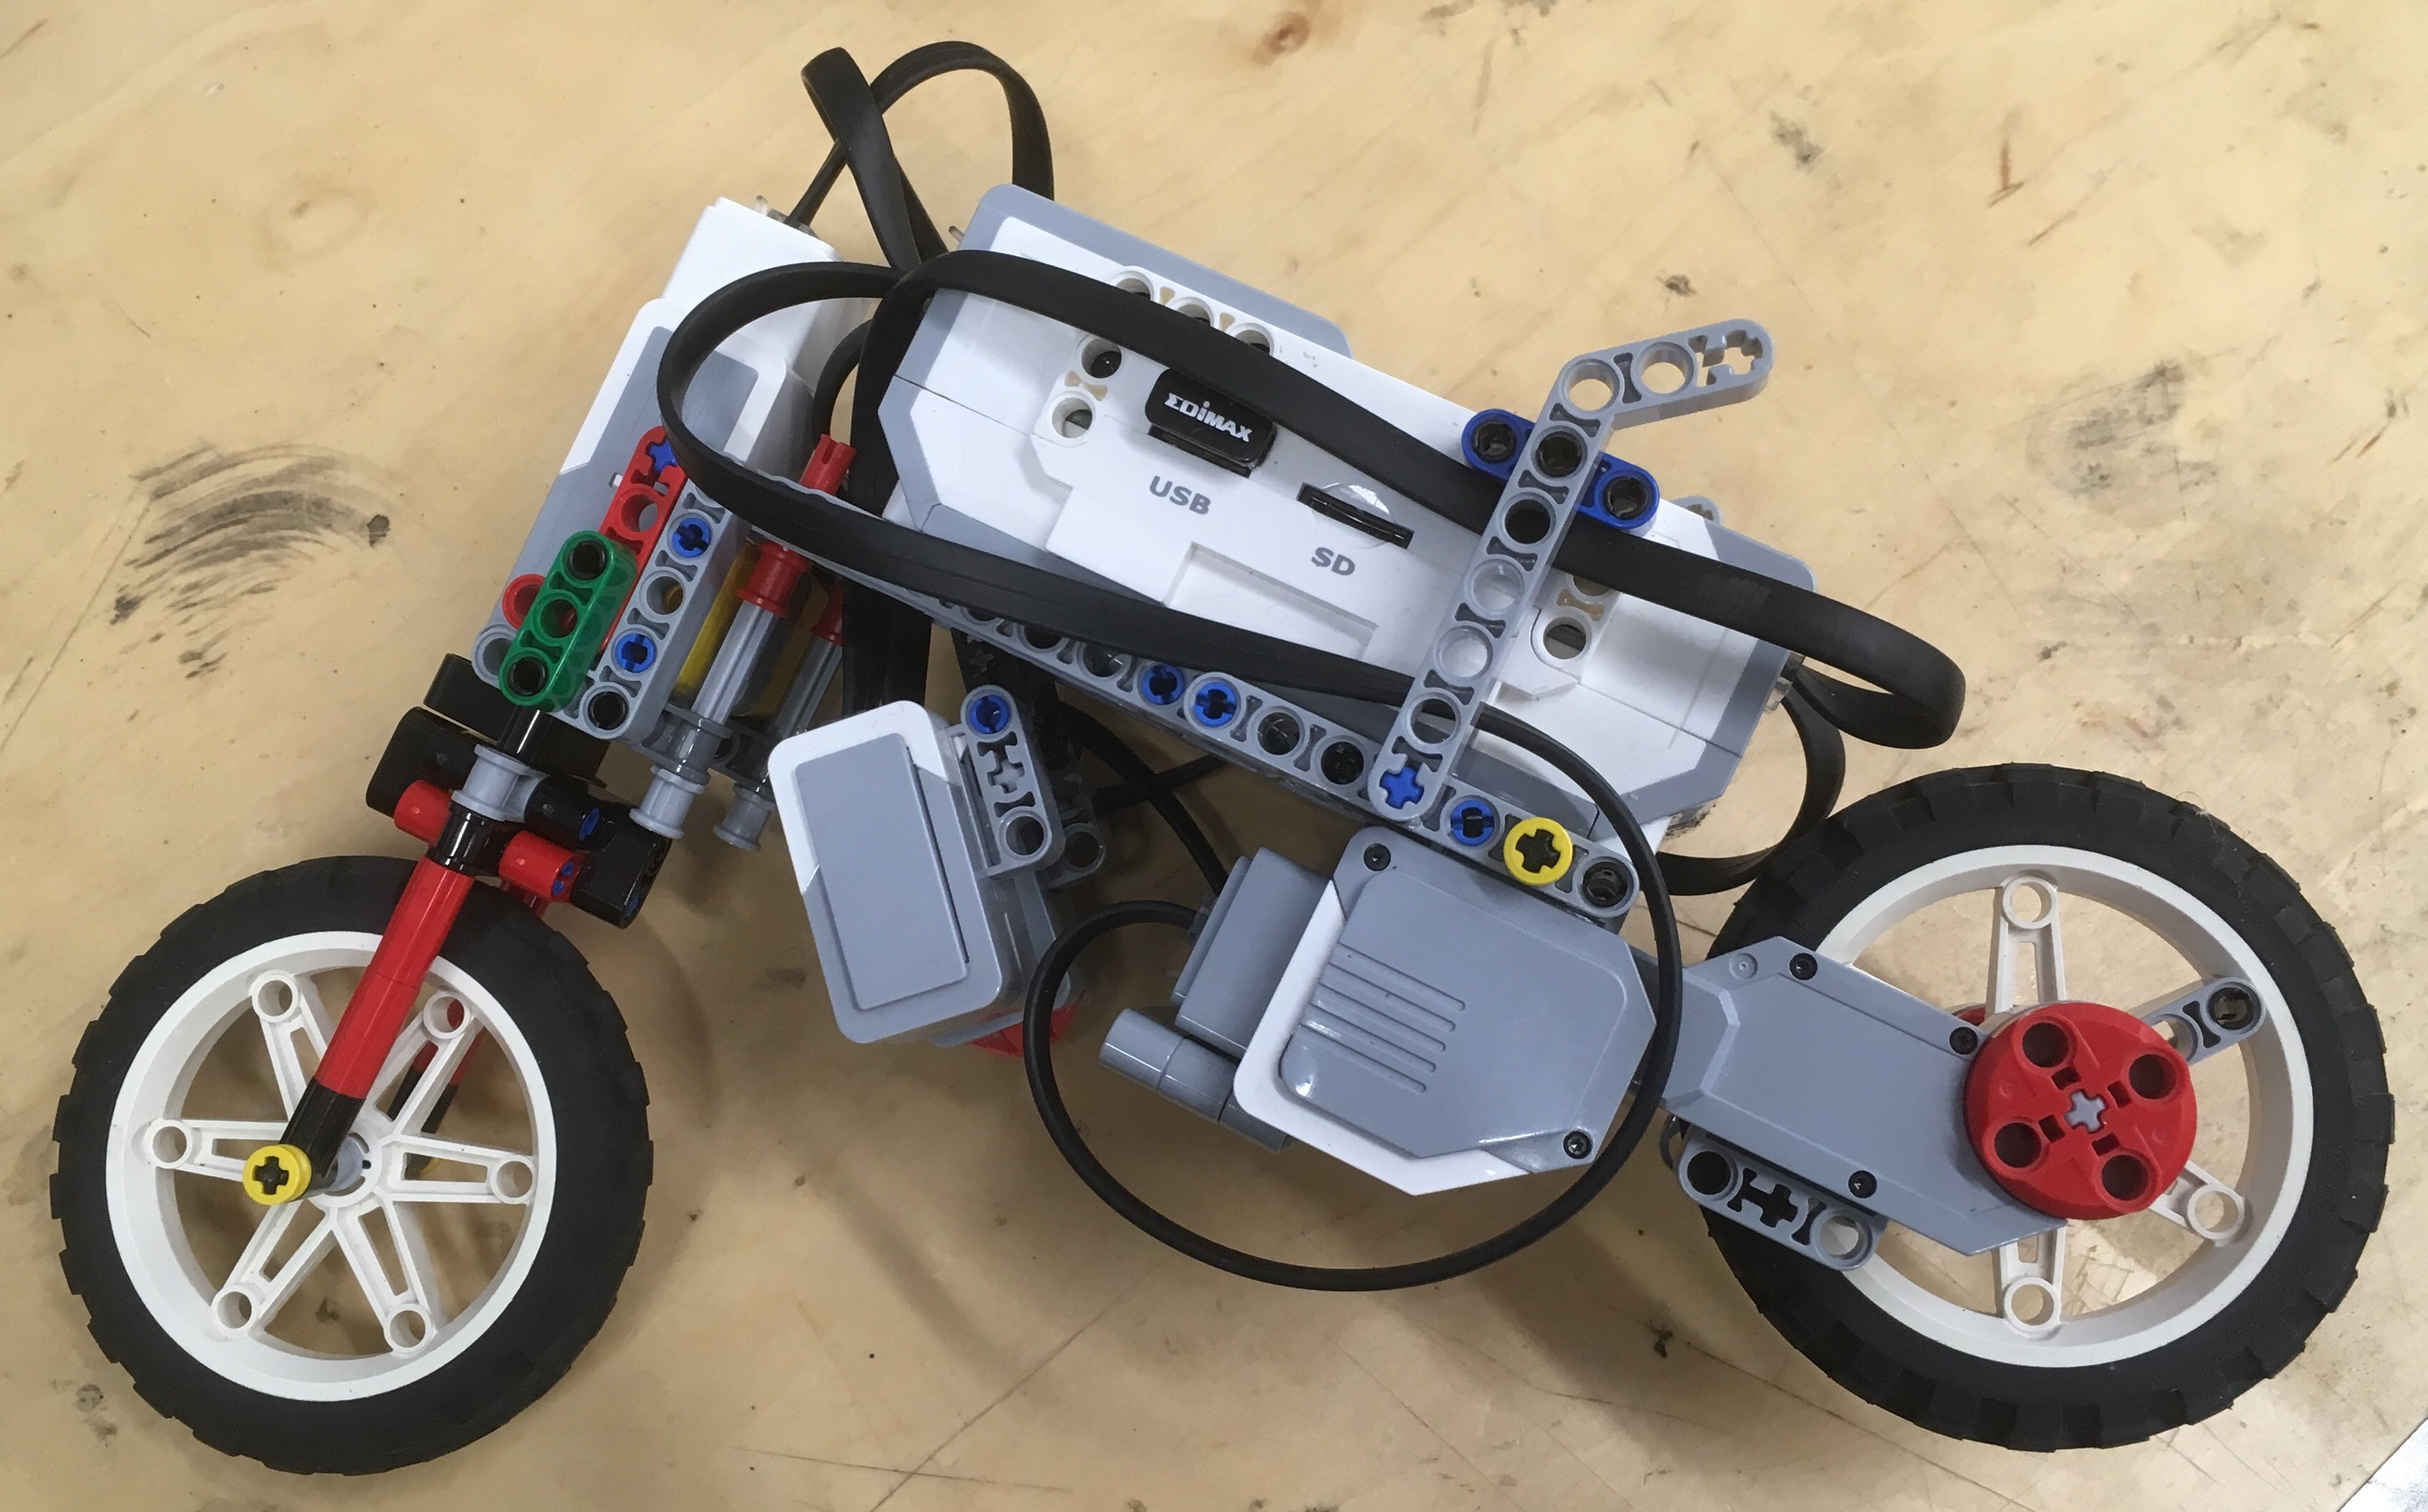
\includegraphics[scale=0.075]{LegoBike.jpg}
\caption{Lego Prototype Bicycle}
\end{figure}

\subsection{Hardware}
Two drive motors to give maximum speed (to aid stability), limited by single gyro sensor (measuring rate of change of lean angle), limited by maximum speed

\subsection{Software}
RobotC, Choice of sample time (dependent on bandwidth of system)

\subsubsection{Lean Angle Estimation}
The Lego bicycle is only equipped with a gyroscopic sensor, meaning that only the rate of change of the lean angle is directly measurable. Direct integration of this measurement to give an estimate of the lean angle is not possible, since the measurements are corrupted by noise and the gyro has a time-varying bias. This noise and gyro bias will cause a drift in the estimated lean angle over time and thus deviate quickly from the true lean angle. Therefore, it is necessary to estimate the lean angle at every timestep using a continuous-discrete \textit{Extended Kalman Filter} (EKF). The EKF fuses the approximately-known, linearised, continuous system dynamics with discrete, noisy sensor readings to give an overall improved state estimate. The state vector and model dynamics are taken from the fourth-order linearised model given in section \ref{FourthOrder}. Note that this entire state estimation step would not be necessary if an accelerometer were available, which could be used as reference to correct for drift. \\

The continuous-discrete EKF can be divided into two steps. Firstly, the \textit{prediction} step uses the system dynamics to estimate the state vector a timestep $T$ in the future:
\begin{align*}
\hat{\underline{x}} &= \hat{\underline{x}} + T \cdot \mathbf{A} \\
\mathbf{P} &= \mathbf{P} + T \cdot (\mathbf{A P} + \mathbf{P} \mathbf{A}^T + \mathbf{Q})
\end{align*}

Where $\hat{\underline{x}}$ is the state estimate vector, $\mathbf{A}$ is the linearised state-transition matrix, $\mathbf{P}$ is the error covariance matrix, and $\mathbf{Q}$ is the model noise matrix. \\

Following this, the \textit{update} step fuses the linearised dynamics with the noisy sensor readings:
\begin{align*}
\mathbf{K} &= \mathbf{P} \mathbf{C}^T (\mathbf{R} + \mathbf{C} \mathbf{P} \mathbf{C}^T)^{-1} \\
\mathbf{P} &= (\mathbf{I} - \mathbf{K C}) \mathbf{P} \\
\hat{\underline{x}} &= \hat{\underline{x}} + \mathbf{K} (\underline{y} - h(\hat{\underline{x}}, \underline{u}))
\end{align*}

Where $h(\hat{\underline{x}}, \underline{u})$ is the output function, $\mathbf{C}$ is the Jacobian of the output function, $\mathbf{R}$ is the measurement noise matrix, and $\mathbf{K}$ is the Kalman gain, which effectively weights the measurements and internal model predictions. \\

Lastly, it is important to note that an approximate model of the dynamics is used in conjunction with a noisy, biased sensor. Even though the resulting state estimation performance is much improved over using only the gyroscope readings, the inevitable inaccuracies will accumulate and degrade the lean angle as time progresses. This of course has a direct impact on control performance and also only allows the final system to be tested for short periods of time before requiring a reset.

\subsubsection{Discrete Form of PID}
To be able to implement a PID controller in software, the continuous-time transfer function needs to be transformed into discrete-time. This is achieved by using the Tustin (Bilinear) transform, which gives the best possible match in the frequency domain between continuous and discrete forms. Furthermore, stability is preserved between the mappings. We start with the transfer function of a \textit{parallel} type PID representation:
\begin{equation*}
K_a(s) = K_P + \frac{K_I}{s} + K_D \frac{s}{s \tau + 1}
\end{equation*}

To discretize this transfer function, we now apply the Tustin mapping from the s to the z-domain:
\begin{equation*}
s \rightarrow \frac{2}{T} \frac{z - 1}{z + 1}
\end{equation*}

Where $T$ is the sample time in seconds. After substituting and rearranging, this leads us to the discrete transfer function representation of the PID controller:
\begin{equation*}
K_d(z) = K_P + K_I \frac{T (z + 1)}{2 (z - 1)} + K_D \frac{2 (z - 1)}{z(2 \tau + T) - (2 \tau - T)}
\end{equation*}

The terms are intentionally kept separated, as in software these can be seen as three distinct blocks which are then summed to give the controller output. The discrete integrator and differentiator can then be implemented simply by difference equations with constant coefficients (assuming a constant sample time $T$).

Integrator wind-up is prevented by clamping. The output is also clamped to prevent the actuator from moving beyond fixed limits.

\subsection{Results}
\subsubsection{Proportional Controller}
A proportional-only controller was indeed able to stabilise the bicycle. As predicted by the second-order model and simulation, the bicycle could be stabilised at the given forward speed of $V=0.44ms^{-1}$ by a gain greater than 11.4. \\
Figures \ref{fig:LegoPController} a) and b) show an excerpt of the response and controller effort of the Lego prototype for a proportional gain of $K_P=12$.

\begin{figure}[H]
	\begin{subfigure}{0.5\textwidth}
	\begin{tikzpicture}
		\begin{axis}
			[xlabel=Time (s),
			 ylabel=Lean Angle $\phi$ (deg),			 
			 xmin=0,xmax=4,
			 ymin=-8,ymax=8,
			 tick label style={/pgf/number format/fixed}]
			\addplot[mark=none] table[x=t,y=phi, col sep=comma] {legoP12.csv};		
		\end{axis}
	\end{tikzpicture}
	\caption{Lean Angle Response}
	\end{subfigure} \hspace{1mm}
	\begin{subfigure}{0.5\textwidth}
	\begin{tikzpicture}
		\begin{axis}
			[xlabel=Time (s),
			 ylabel=Steering Angle $\delta$ (deg),
			 xmin=0,xmax=4,
			 ymin=-75,ymax=75,
			 legend pos=north west,
			 tick label style={/pgf/number format/fixed}]
			\addplot[mark=none,color=red] table[x=t,y=delta, col sep=comma] {legoP12.csv};			
		\end{axis}
	\end{tikzpicture}
	\caption{Actuator Effort}
	\end{subfigure}
	\caption{P-Controller Response ($K_P=12$)}
	\label{fig:LegoPController}
\end{figure}

The response for the simple proportional controller is certainly not ideal, even though stability is achieved.  The magnitude of the lean angle is bounded by approximately $5^{\circ}$, which is an acceptable deviation from the desired setpoint of $0^{\circ}$. However, there is an oscillation present in the response, indicating that the system is on the boundary of stability. Knocking the bicycle gently, as to add an output disturbance, destabilises it. Thus the closed-loop system is not robust and sensitive to disturbances in its current state. This is to be expected however, since we are using a proportional gain which places the closed-loop poles very close to the imaginary axis. As shown, inevitable model uncertainties will deteriorate the control performance from the ideal calculations and simulations. Furthermore, this \textit{jittering} behaviour also causes the bicycle to move off-track easily and not follow a straight path. Lastly, the controller effort is larger than ideal. However, this large actuator command is required for stability. \\

As a brief aside, the servo model is again verified by running a simulation in Matlab but using the real-world controller output data. As can be seen in Figure \ref{fig:LegoServoIDPart2}, the match is near perfect and confirms the actuator model identified in an earlier section of this report. \\

\begin{figure}[H]
\centering
\begin{tikzpicture}
		\begin{axis}
			[xlabel=Time (s),
			 ylabel=Steering Angle $\delta$ (deg),
			 xmin=0,xmax=4,
			 ymin=-75,ymax=75,
			 legend pos=north west,
			 tick label style={/pgf/number format/fixed}]
			\addplot[mark=none,dashed] table[x=t,y=delta, col sep=comma] {legoP12.csv};
			\addplot[mark=none,color=blue] table[x=t, y=deltasim, col sep=comma] {legoP12.csv};
		\end{axis}
	\end{tikzpicture}
	\caption{Lego Servo Model Verification}
	\label{fig:LegoServoIDPart2}
\end{figure}

\subsubsection{Proportional-Derivative Controller}
As a next step, we will aim to improve control performance by adding phase lead to the controller, as discussed in the section on controller design. This is achieved by the use of a lead compensator.  This can also be seen as a parallel combination of a proportional gain and a band-limited differentiator. The lead compensator increases the phase margin of the system in the hope of reducing the oscillations currently present in the closed-loop response. HOW DO WE SPLIT THIS BETWEEN CONTROLLER DESIGN AND IMPLEMENTATION??? \\

\begin{equation}
K_{Lead}(s) = 14 \cdot \frac{s + 1.1}{s + 2.0}
\end{equation}

Or in PD form,

\begin{equation}
K_{PD}(s) = 8 + 3 \frac{s}{s \cdot 0.50 + 1}.
\end{equation}
\begin{figure}[H]
	\begin{subfigure}{0.5\textwidth}
	\begin{tikzpicture}
		\begin{axis}
			[xlabel=Time (s),
			 ylabel=Lean Angle $\phi$ (deg),			 
			 xmin=0.25,xmax=2.5,
			 ymin=-1.5,ymax=1.5,
			 tick label style={/pgf/number format/fixed}]
			\addplot[mark=none] table[x=t,y=phi, col sep=comma] {legoPDData.csv};
		\end{axis}
	\end{tikzpicture}
	\caption{Lean Angle Response}
	\end{subfigure} \hspace{1mm}
	\begin{subfigure}{0.5\textwidth}
	\begin{tikzpicture}
		\begin{axis}
			[xlabel=Time (s),
			 ylabel=Steering Angle $\delta$ (deg),
			 xmin=0.25,xmax=2.5,
			 ymin=-15,ymax=15,
			 legend pos=north west,
			 tick label style={/pgf/number format/fixed}]
			\addplot[mark=none,color=red] table[x=t,y=delta, col sep=comma] {legoPDData.csv};			
		\end{axis}
	\end{tikzpicture}
	\caption{Actuator Effort}
	\end{subfigure}
	\caption{PD-Controller Response ($K_P=8$, $K_D=3$, $\tau=0.5$)}
	\label{fig:LegoP12Controller}
\end{figure}

Small oscillations still remain but better damped , controller effort is greatly reduced for a better performance! Derivative is heavily filtered (tau=0.5), so that the jiterring which would otherwise occur due to noise is redueced. Lean angle only just above 1 deg.

\subsubsection{Final Observations}
hard to stabilise since h is small and time constants are short, not robust to disturbances. Have hardly any time to react. Additional limitation is maximum speed of lego model, which causes it to be very unstable. Stabilisation can be achieved but not a very good performance. Performance could probably be improved if we were to use a better angle estimation system, i.e. use an IMU. As soon as gyro estimate starts drifting we're in trouble (which turns out to be pretty quickly)...